% TEX-option: shell-escape

\documentclass[a4paper,11pt]{article}

\usepackage[
    backend=biber,
    style=numeric,
    sortlocale=de_DE,
    natbib=true,
    url=false, 
    doi=true,
    eprint=false
]{biblatex}

\usepackage[left=3.0cm, right=3.0cm, top=2.5cm, bottom=2.5cm]{geometry}
\usepackage{url}
\usepackage{menukeys}
\usepackage{cleveref}
\usepackage{graphicx}
\usepackage[disable]{todonotes}
\usepackage{upgreek}
\usepackage{dirtree}
\usepackage[nonumberlist]{glossaries}
\usepackage[autostyle]{csquotes}

\usepackage[parfill]{parskip}

\usepackage{listings} % Syntax highlighting
\lstset{
  breaklines=true,                
  basicstyle=\ttfamily,
  showstringspaces=false,
  commentstyle=\color{red},
  keywordstyle=\color{blue},
  columns=fullflexible
}

% Python style for highlighting
\lstdefinestyle{MyPython}{
language=Python,
basicstyle=\ttm,
otherkeywords={self},             % Add keywords here
keywordstyle=\ttb\color{deepblue},
emph={MyClass,__init__},          % Custom highlighting
emphstyle=\ttb\color{deepred},    % Custom highlighting style
stringstyle=\color{deepgreen},
frame=tb,                         % Any extra options here
showstringspaces=false            % 
}

\usepackage{syntax}
\setlength{\grammarparsep}{20pt plus 1pt minus 1pt} % increase separation between rules
\setlength{\grammarindent}{12em} % increase separation between LHS/RHS 



\newcommand{\token}[1]{\lstinline$#1$}
\newcommand{\myparagraph}[1]{\paragraph{#1}\mbox{}}

% Glossary

\makeglossaries
%Term definitions
\newglossaryentry{ast}{name=AST, description={Abstract Syntax Tree}}
\newglossaryentry{bnf}{name=BNF, description={Backus-Naur Form}}
\newglossaryentry{lalr}{name=LALR, description={Look-Ahead Left to Right, Rightmost derivation parser}}
\newglossaryentry{tdd}{name=TDD, description={Test-driven development}}
\renewcommand*{\glossaryname}{List of Abbreviations}

% Bibliography

\addbibresource{bibliography.bib}

%Autornamen in Bibliography fett
\AtBeginBibliography{\renewcommand*{\mkbibnamelast }[1]{\textbf{#1}}}
\AtBeginBibliography{\renewcommand*{\mkbibnamefirst }[1]{\textbf{#1}}}

% Hyperref

\usepackage{hyperref}
\hypersetup{colorlinks=false}

% BEGIN DOCUMENT

\begin{document}

\pagenumbering{roman}

%!TEX root = ../main.tex
%%%%%%%%%%%%%%%%%%%%%%%%%%%%%%%%%%%%%%%%%
% University Assignment Title Page 
% LaTeX Template
% Version 1.0 (27/12/12)
%
% This template has been downloaded from:
% http://www.LaTeXTemplates.com
%
% Original author:
% WikiBooks (http://en.wikibooks.org/wiki/LaTeX/Title_Creation)
%
% License:
% CC BY-NC-SA 3.0 (http://creativecommons.org/licenses/by-nc-sa/3.0/)
% 
% Instructions for using this template:
% This title page is capable of being compiled as is. This is not useful for 
% including it in another document. To do this, you have two options: 
%
% 1) Copy/paste everything between \begin{document} and \end{document} 
% starting at \begin{titlepage} and paste this into another LaTeX file where you 
% want your title page.
% OR
% 2) Remove everything outside the \begin{titlepage} and \end{titlepage} and 
% move this file to the same directory as the LaTeX file you wish to add it to. 
% Then add \input{./title_page_1.tex} to your LaTeX file where you want your
% title page.
%
%%%%%%%%%%%%%%%%%%%%%%%%%%%%%%%%%%%%%%%%%

%----------------------------------------------------------------------------------------
%	PACKAGES AND OTHER DOCUMENT CONFIGURATIONS
%----------------------------------------------------------------------------------------

\begin{titlepage}

\newcommand{\HRule}{\rule{\linewidth}{0.5mm}} % Defines a new command for the horizontal lines, change thickness here

\center % Center everything on the page
 
%----------------------------------------------------------------------------------------
%	HEADING SECTIONS
%----------------------------------------------------------------------------------------

\textsc{\LARGE DHBW Mannheim}\\[1.5cm] % Name of your university/college
\textsc{\Large Student research project}\\[0.5cm] % Major heading such as course name
\textsc{\large TINF11AI-BC}\\[0.5cm] % Minor heading such as course title

%----------------------------------------------------------------------------------------
%	TITLE SECTION
%----------------------------------------------------------------------------------------

\HRule \\[0.4cm]
{ \huge \bfseries Implementing a SetlX to Pyton compiler}\\[0.4cm] % Title of your document
\HRule \\[1.5cm]
 
%----------------------------------------------------------------------------------------
%	AUTHOR SECTION
%----------------------------------------------------------------------------------------

\begin{minipage}{0.4\textwidth}
\begin{flushleft} \large
\emph{Author:}\\
Jan-Christoph \textsc{Klie} % Your name
\end{flushleft}
\end{minipage}
~
\begin{minipage}{0.4\textwidth}
\begin{flushright} \large
\emph{Supervisor:} \\
Prof. Dr. Karl \textsc{Stroetmann} % Supervisor's Name
\end{flushright}
\end{minipage}\\[4cm]

% If you don't want a supervisor, uncomment the two lines below and remove the section above
%\Large \emph{Author:}\\
%John \textsc{Smith}\\[3cm] % Your name

%----------------------------------------------------------------------------------------
%	DATE SECTION
%----------------------------------------------------------------------------------------

{\large \today}\\[3cm] % Date, change the \today to a set date if you want to be precise

%----------------------------------------------------------------------------------------
%	LOGO SECTION
%----------------------------------------------------------------------------------------

%\includegraphics{Logo}\\[1cm] % Include a department/university logo - this will require the graphicx package
 
%----------------------------------------------------------------------------------------

\vfill % Fill the rest of the page with whitespace

\end{titlepage}

\tableofcontents
\clearpage
%\listoftables
\listoffigures
\printglossaries

\pagenumbering{arabic}

% ************************
% USER GUIDE
% ************************
\clearpage
\part{User Guide}

<<<<<<< HEAD
%!TEX root = ../main.tex

\section{Preface}

\subsection{Overview}

Setlx2py consists of two parts: It is a compiler written in the Python programming language to transcompile SetlX sources to Python. In addition to that, it contains the needed runtime libraries. Therefore, when running code generated by setlx2py, an installed setlx2py environment is needed. When the development of setlx2py comes to a stable, binaries for the different target architectures are created simplify the step of installation.

In the following chapters, the steps needed to setup setlx2py on your system are described. It can be run on nearly any platform which has a standard Python implementation. At first, the general dependencies are described. After that, some in-depth guides for installing on Windows, Ubuntu Linux and Mac OS can be found. In the end, the actual usage of setlx2py is briefly explained.

\subsection{Dependencies}

To deal with a target platform which is not described here, or this installation guide becomes outdated, the dependencies necessary to run setlx2py are now explained.

\paragraph{Runtime}

Setlx2py is written in Python, and generates Python source code from SetlX input. Therefore, a Python runtime is needed. Any version starting from Python 2.7 is officially supported. It tested with version numbers 2.7 and 3.3. Older versions may work, but are not recommended nor supported.

\paragraph{Packages}

\begin{itemize}
\item PLY \footnote{\url{https://pypi.python.org/pypi/ply}}
\item blist \footnote{\url{https://pypi.python.org/pypi/blist}}
\item nose (only for testing) \footnote{\url{https://pypi.python.org/pypi/nose}}
\item ast-gen (only for development) \footnote{\url{https://github.com/Rentier/ast-gen}}
=======
\section{Preface}

\subsection{Overview}

Setlx2py consists of two parts: It is a compiler written in the Python programming language to transcompile SetlX sources to Python. In addition to that, it contains the needed runtime libraries. Therefore, when running code generated by setlx2py, an installed setlx2py environment is needed. 

In the following chapters, the steps needed to setup setlx2py on your system are described. It can be run on nearly any platform which has a standard Python implementation. At first, the general dependencies are described. After that, some in-depth guides for installing on Windows, Ubuntu Linux and Mac OS can be found. In the end, the actual usage of setlx2py is briefly explained.

\subsection{Dependencies}

To deal with a target platform which is not described here, our this installation guide becomes outdated, the dependencies necessary to run setlx2py are now explained.

\paragraph{Runtime}

Setlx2py is written in Python, and generates Python source code from SetlX input. Therefore, a Python runtime is needed. Any version starting from Python 2.7 is officially supported. It tested with version numbers 2.7 and 3.3. Older versions may work, but are not recommended nor supported.

\paragraph{Packages}

\begin{itemize}
\item PLY \footnote{\url{https://pypi.python.org/pypi/ply}}
\item blist \footnote{\url{https://pypi.python.org/pypi/blist}}
\item nose (only for testing) \footnote{\url{https://pypi.python.org/pypi/nose}}
\item ast-gen (only for development) \footnote{\url{https://github.com/Rentier/ast-gen}}
>>>>>>> 6640584894f5245d515ca7633dadcb0b4d99f7b3
\end{itemize}
%!TEX root = ../main.tex
\section{Windows}

\subsection{Install Python}

\subsubsection{Obtain the Python binary}

First, download a Python installer from the official Website, which can be found at \url{https://www.python.org/download/}. Be sure to select an installer, not source packages. It should not matter which version you use, but recommended is the either the newest version of 2.7 or the newest version of 3.X. It is a matter of taste, and might depend on which version you might already have installed. But setlx2py should run with all newer versions of standard Python.

The setup itself is self-explanatory, just run the executable as usual. When you decide where to install, it is recommended to let Python install where it wants. If you choose a different installation path, remember where it was, you will need that information in the next step. The location of the Python installation is called \texttt{\$PYHOME} for further reference.

\subsubsection{Setting the \$PATH}

Now you could run Python with the command

\begin{lstlisting}{breaklines=true, language=bash}
# $PYHOME\python.exe
\end{lstlisting}

Typing the full path is very tedious. To ease the usage of the Python interpreter, Windows has the feature of the \texttt{\$PATH}-Variable. Whenever you insert a command without a fully specified path, it looks in the folders you specified in that variable, and looks for a match. There are two ways to add a program to the path variable. Open a Powershell with either \keys{Win + R + "powershell" + Enter}. Insert the follwing command in the just opened window: 

\begin{lstlisting}{breaklines=true, language=bash}
# [Environment]::SetEnvironmentVariable("Path", "$env:Path;C:\Python27\;C:\Python27\Scripts\", "User")
\end{lstlisting}

In that example, we used Python 2.7. If you installed another version of python, or used a different \texttt{\$PYHOME}, adjust the part of \textit{C:\textbackslash Python27} to reflect the differences. 

Close the shell and open it again. You should now be able to open a Python prompt with entering

\begin{lstlisting}{breaklines=true, language=bash}
# python
\end{lstlisting}

in the shell. 

\begin{figure}[ht]
    \centering
    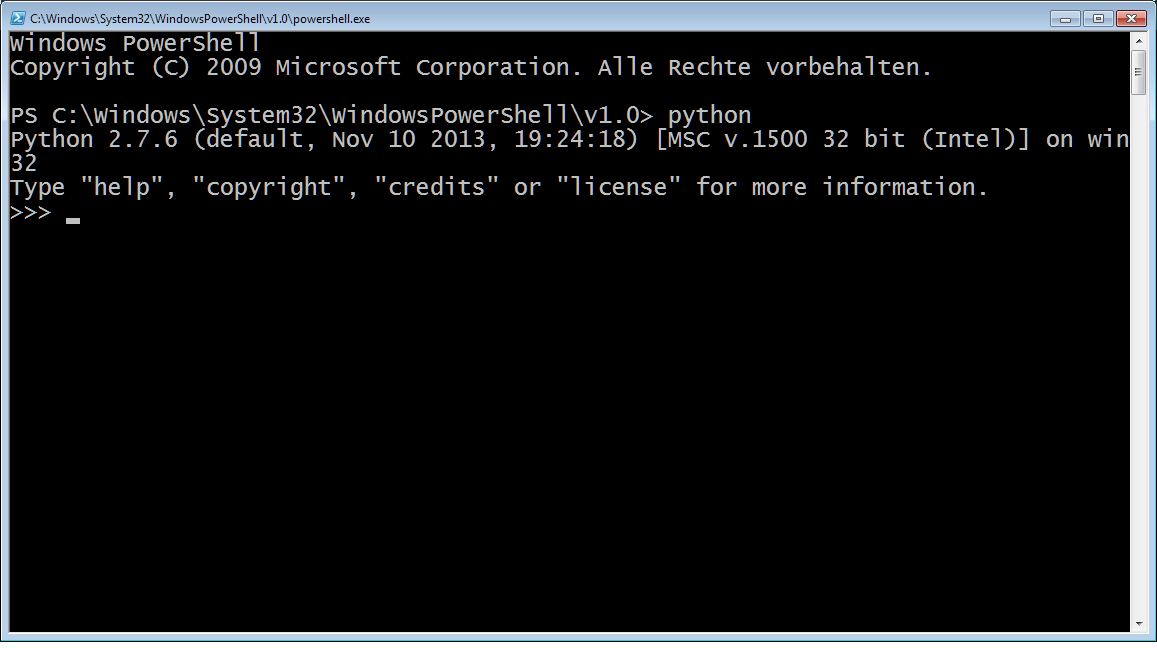
\includegraphics[width=0.8\textwidth]{img/install-python.png}
    \caption{Running python from a shell without fully specified path}
    \label{fig:install-python}
\end{figure}

\subsection{Install package manager}

Python allows installing packages in a very easy way. Sadly, it does not ship with a package manager. Therefore, it is installed in the next step. Download

\url{https://raw.github.com/pypa/pip/master/contrib/get-pip.py}

Open a shell and change the directory to the folder to where you downloaded it (the \keys{cd + \$FOLDERNAME} command does that for you). Now run 

\begin{lstlisting}{breaklines=true, language=bash}
# python \.get-pip.py
\end{lstlisting}

You should see a confirmation that it is installed everything successfully like in Fig. \ref{fig:install-pip}.

\begin{figure}[ht]
    \centering
    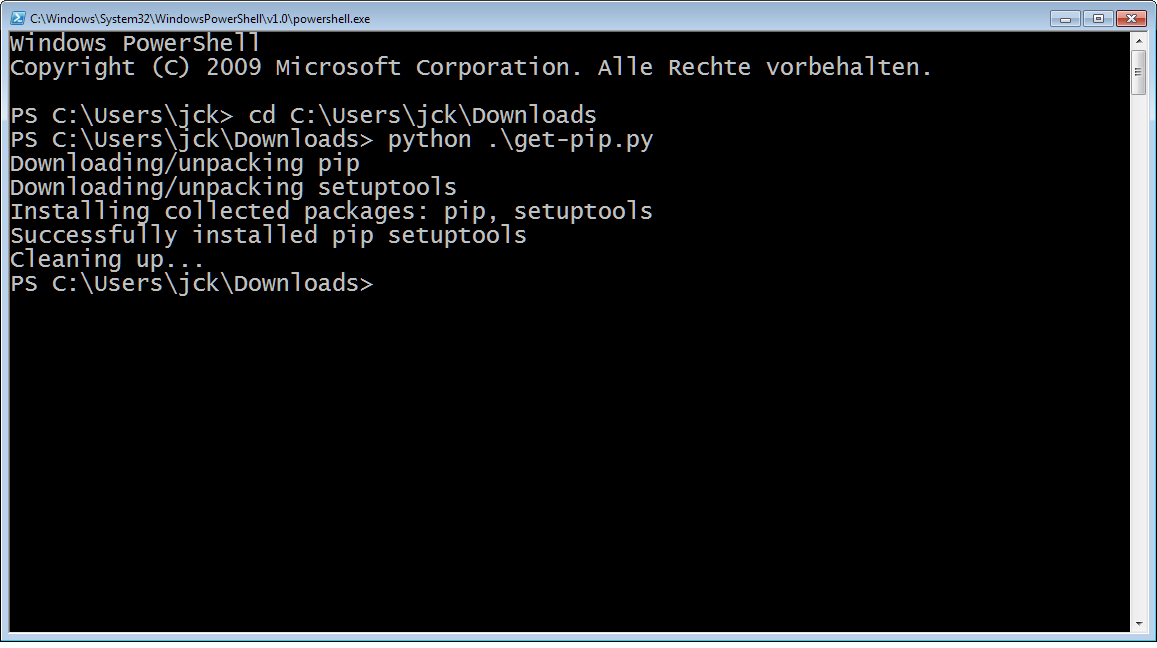
\includegraphics[width=0.8\textwidth]{img/install-pip.png}    
    \caption{Installing the package manager pip}
    \label{fig:install-pip}    
\end{figure}

\subsection{Install binary dependencies}

Setlx2py uses internally some platform-specific binary libraries. It is possible to compile these for Windows with some effort, but people offer them precompiled already. Download the fitting version of the \texttt{blist} package (for the curious, it offers better/more advanced data structures) and install it. Be sure to download the same architecture as you did for Python (32- or 64-bit), else you get an error with a name of "Cannot install" or similar. The package itself can be obtained from

\url{http://www.lfd.uci.edu/~gohlke/pythonlibs/#blist}

\subsection{Install dependencies}

Download the setlx2py archive from 

\url{https://github.com/Rentier/setlx2py/archive/master.zip}

and extract it. Open a shell and change the working directory to the folder where the \texttt{REQUIREMENTS.txt} file can be found. With the power of \texttt{pip}, all other dependencies can now be installed with 

\begin{lstlisting}{breaklines=true, language=bash}
# pip install -r REQUIREMENTS.txt
\end{lstlisting}

The package manager now retrieves all the dependencies specified in the given file. After some time, it messages "Successfully installed". Everything is now in place to actually use setlx2py.

\begin{figure}[ht]
    \centering
    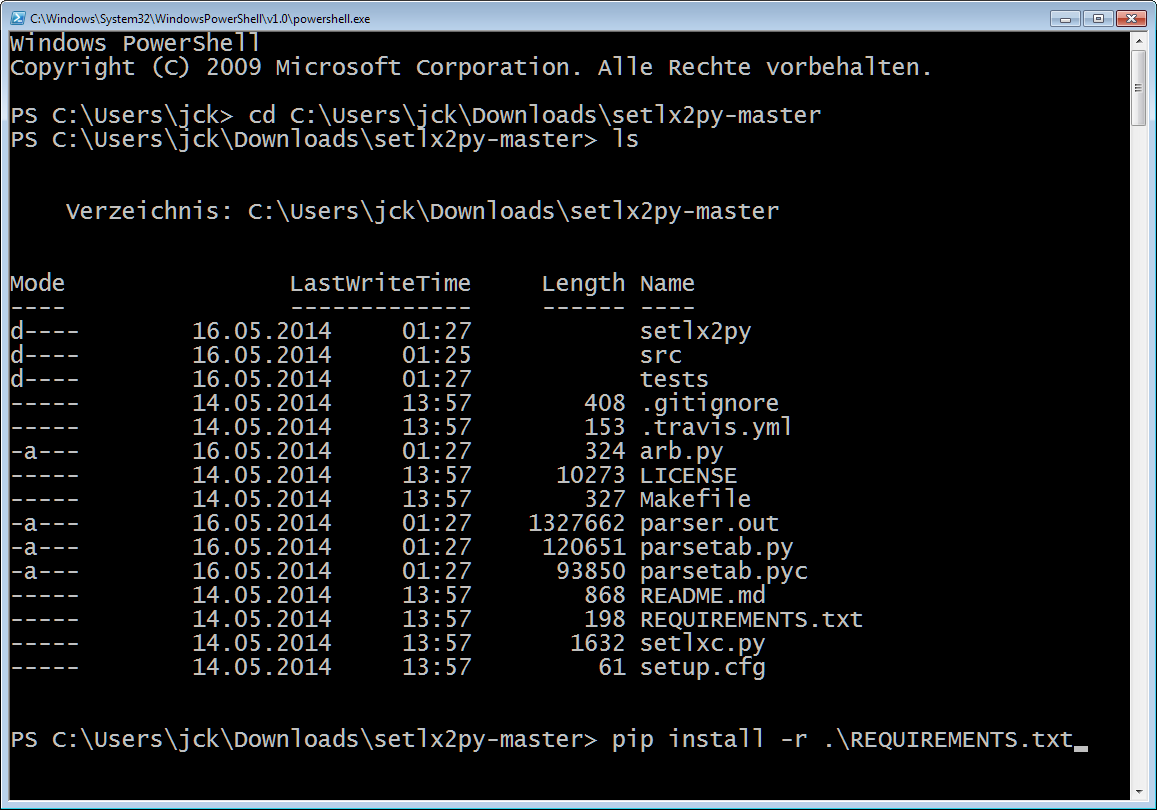
\includegraphics[width=0.8\textwidth]{img/install-reqs.png}
    \caption{Installing the dependencies of setlx2py with pip}
    \label{fig:install-req}
\end{figure}

\subsection{Use setlx2py}

Now that all prequisites are installed, the actual compiler can be downloaded. This step uses the previously installed package manager, so it only requires one command to install setlx2py. Grab an open shell, and issue the following command:

\begin{lstlisting}{breaklines=true, language=bash}
# pip install git+git://github.com/Rentier/setlx2py.git@master
\end{lstlisting}
%!TEX root = ../main.tex

\section{Usage}

Using setlx2py consists of two steps. At first, one has to compile a given SetlX source file. That can be done with

\begin{lstlisting}{breaklines=true, language=bash}
$ setlxc.py -i STLX_IN -o PY_OUT
\end{lstlisting}

where \texttt{STLX\_IN} is the path to the SetlX source file, and \texttt{PY\_OUT} the path to the file where the Python code will be saved.

The generated file then has to be run with the Python interpreter:

\begin{lstlisting}{breaklines=true, language=bash}
$ python PY_OUT
\end{lstlisting}

The complete steps can be seen in the Fig. \ref{fig:use-sieve}.

\begin{figure}[ht]
    \centering
    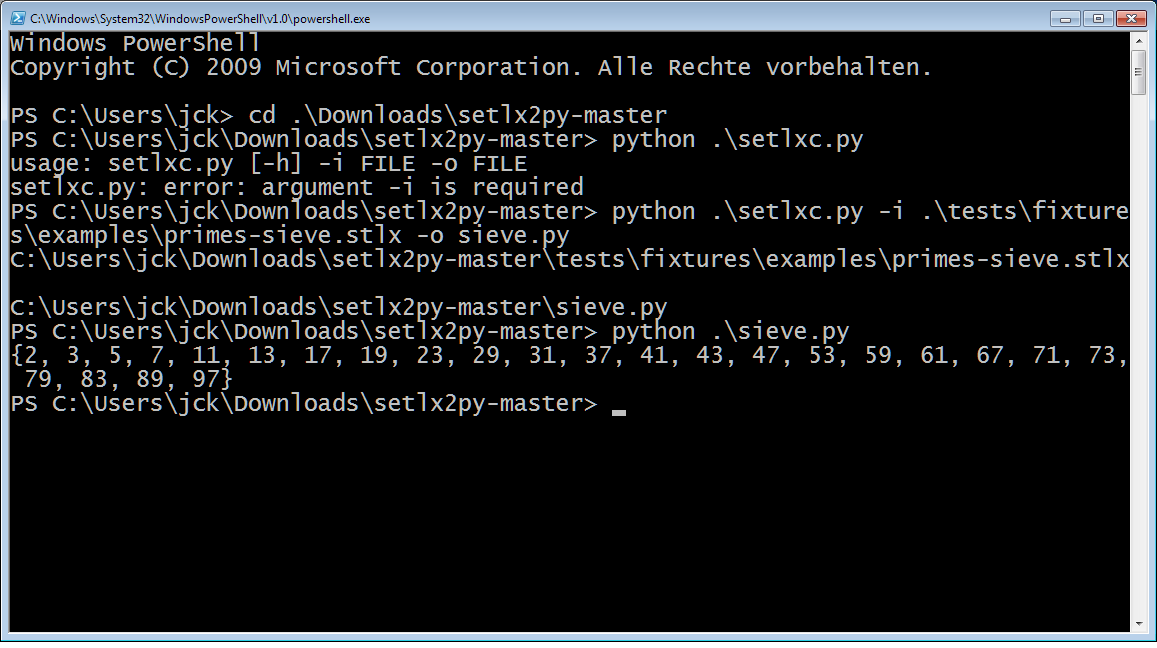
\includegraphics[width=0.8\textwidth]{img/sieve.png}
    \caption{Using setlx2py to compile SetlX and running the generated Python}
    \label{fig:use-sieve}
\end{figure}

%\section{Linux}

%\section{Mac OS}

% ************************
% LANGUAGE REFERENCE
% ************************
\clearpage
\part{The SetlX language}
\clearpage

%!TEX root = ../main.tex
\section{Lexical analysis}

The following chapter describes the tokens used in setlx2py. The model used is heavily borrowed from the one Python 2.7. It can be found in \cite{py2}.

%
% SUBSECTION
%
\subsection{Line structure}

A SetlX program is built of logical lines.

%#####################
%
\subsubsection{Logical lines}

The end of a logical line is represented by a semicolon `;'.

%#####################
%
\subsubsection{Physical lines}

A physical line consists of a number of characters ending with a end-of-line character. One physical line can have any fraction of a logical line, i.e. one can split code arbitrarily at whitespace.

%#####################
%
\subsubsection{Comments}

Setlx has two types of comments. Comments are ignored by the lexer, they are stripped and do not generate any tokens.

\myparagraph{Singe-line comments}

A single line comment starts with a double slash (\token{//}) that is not part of a string literal, and ends at the end of the physical line. 

\myparagraph{Multi-line comments}

Multi-line comments, start with \token{/*} and end with \token{*/}.

%#####################
%
\subsubsection{Blank lines}

Lines that only contain whitespace are ignored.

%#####################
%
\subsubsection{Whitespace}
Except in string literals, the whitespace characters used to separate tokens are tab, carriage return, form feed, vertical tab.

%
% SUBSECTION
%
\subsection{Identifiers and keywords}

Identifier and functors are unlimited in length. Case is significant.

%#####################
%
\subsubsection{Identifier}

Identifiers are described by the following lexical definitions:

\begin{grammar}
<identifier> ::= <lowercase> <seq> | `_'

<seq> ::= <seq> <char>
\alt $\upepsilon$

<char> ::= <lowercase> | <uppercase> | <digit> | `_'

<lowercase>  ::=  `a'...`z'

<uppercase>  ::=  `A'...`Z'

<digit>      ::=  `0'...`9'
\end{grammar}

%#####################
%
\subsubsection{Functor}

Functors are described by the following lexical definitions:

\begin{grammar}
<functor> ::= <uppercase> <seq>
\end{grammar}

%
% SUBSECTION
%
\subsection{Keywords}

The following identifier are treated as keywords in SetlX and cannot used for other purposes:

\begin{table}[h]
\begin{tabular*}{\columnwidth}{@{\extracolsep{\stretch{1}}}*{6}{l}@{}}
\token{true} 		& \token{false} 			& \token{in} 		& \token{notin} 	& \token{forall} 	& \token{exists} 	\\
\token{backtrack} 	& \token{check} 			& \token{match} 	& \token{regex} 	& \token{as} 		& \token{break} 	\\
\token{continue} 	& \token{exit} 				& \token{return} 	& \token{assert} 	& \token{if} 		& \token{else} 		\\
\token{switch} 		& \token{case} 				& \token{default} 	& \token{for} 		& \token{do} 		& \token{while} 	\\
\token{procedure} 	& \token{cachedProcedure} 	& \token{class} 	& \token{static} 	& \token{scan} 		&  \token{using} 	\\
\token{try} 		&  \token{catch} 			& \token{catchUsr} 	& \token{catchLng} 	&  \\
\end{tabular*}
\end{table}

%
% SUBSECTION
%
\subsection{Literals}

Literals are notations for constant values of some built-in types.

%#####################
%
\subsubsection{Character sequences}

\myparagraph{Strings}

Any sequence of characters enclosed in double quotes which does not contain a interpolation is considered a string.

\myparagraph{Literal strings}

Any sequence of characters enclosed in single quotes is considered a literal string.

\myparagraph{String interpolations}

A string interpolation is a string which contains at least one interpolation.

\begin{grammar}
<interpolation> ::= `\$' <expression> `\$'
\end{grammar}

\myparagraph{Escaping}

SetlX supports the same escape sequences as the language C.

%#####################
%
\subsubsection{Numeric literals}

There are two types of numeric literals: integer and floating point numbers. Note that the following definitions do not include signs, that is handled by expressions with unary operators.

\myparagraph{Integer literals}

\begin{grammar}
<integer> ::=  <nonzerodigit> <digits-or-empty> | `0'

<nonzerodigit>   ::=  `1'...`9'

<digits> ::= <digits> <digit>
\alt <digit>

<digits-or-empty> ::= <digits> | $\upepsilon$
\end{grammar}

\myparagraph{Floating point literals}

Floating point literals are described by the following lexical definitions:

\begin{grammar}
<floatnumber>   ::=  <pointfloat> | <exponentfloat>

<pointfloat>    ::=  <fraction>
\alt <intpart> <fraction>
\alt <intpart> `.'

<exponentfloat> ::=  <significand> <exponent>

<significand> ::= <intpart> | <pointfloat>

<intpart>       ::=  <digits>

<fraction>      ::=  `.' <digits>

<exponent>      ::= <e> <sign> <digits>

<e> ::= `e' | `E'

<sign> ::= `+' | `-' | $\upepsilon$

\end{grammar}

%
% SUBSECTION
%
\subsection{Operators}

The following tokens are operators:

\begin{table}[h]
\begin{tabular*}{\columnwidth}{@{\extracolsep{\stretch{1}}}*{6}{l}@{}}
\token{+} 		& \token{-} 	& \token{/} 	& \token{*} 	& \token{\\\\} 	& \token{\%} \\
\token{><} 		& \token{**} 	& \token{\#} 	& \token{@}	& 						 					& \\
\token{<==>} 	& \token{<!=>}	& \token{=>}	& \token{||}	& \token{\&\&} 								& \token{!} \\
\token{==} 		& \token{!=} 	& \token{<} 	& \token{<=} 	& \token{>} 								& \token{>=} \\
\token{\\+} & \token{\\*} & & & &	\\
\end{tabular*}
\end{table}

%
% SUBSECTION
%
\subsection{Delimiters}

The following tokens serve as delimiters in the grammar:

\begin{table}[h]
\begin{tabular*}{\columnwidth}{@{\extracolsep{\stretch{1}}}*{6}{l}@{}}
\token{(} 	& \token{)} 	& \token{[} 	& \token{]} 	& \token{\{}	& \token{\}} 	\\
\token{;} 	& \token{,} 	& \token{:} 	& \token{..}	& \token{.} 	& \token{|} 	\\
\token{:=}	& \token{+=}	& \token{-=} 	& \token{*=}	& 				&				\\
\token{/=}	& \token{\\=} & \token{\%=} &\token{|->}				\\
\end{tabular*}
\end{table}
%\section{Execution model}
%\subsection{Scoping}
%!TEX root = ../main.tex
\section{Grammar}

In this chapter, the grammar of SetlX is explained. The syntax used to describe it is \gls{bnf}. The grammar was implemented in a \gls{lalr}(1) parser, therefore, the grammar is LALR(1). 

In some cases, the reader might think of an easier way to express given constructs. These strange and too complex looking rules are in most cases written that way to preserve the LALR nature and to deal with parsers which do not offer operator precedence.

\todo{Pyton Grammar}
The grammar model used is heavily borrowed from the Python 2.7 grammar. It can be found in 

%
% SUBSECTION
%
\subsection{Top-level components}

All input read from files has the same form:

\begin{grammar}
<S> ::= <file_input>

<file_input> ::= <statement_list>
\alt <expression>

<statement_list> ::= <statement>
\alt <statement_list> <statement>

<statement> ::= <simple_statement> `;'
\alt <compound_statement>

<block> ::= <statement_list>
\alt $\upepsilon$
\end{grammar}

%
% SUBSECTION
%
\clearpage
\subsection{Expressions}

This section explains the elements occuring in SetlX expressions.

\begin{grammar}
<expression> ::= <implication>
\alt <lambda_definition>
\alt <implication> `<==>' <implication>
\alt <implication> `<!=>' <implication>

<implication> ::= <disjunction>
\alt <disjunction> `=>' <disjunction>

<disjunction> ::= <conjunction>
\alt <disjunction> `||' <conjunction>

<conjunction> ::= <comparison>
\alt <conjunction> `&&' <comparison>

<comparison> ::= <sum>
\alt <sum> `==' <sum>
\alt <sum> `!=' <sum>
\alt <sum> `<' <sum>
\alt <sum> `<=' <sum>
\alt <sum> `>' <sum>
\alt <sum> `>=' <sum>
\alt <sum> `in' <sum>
\alt <sum> `notin' <sum>

<sum> ::= <product>
\alt <sum> `+' <product>
\alt <sum> `-' <product>

<product> ::= <reduce>
\alt <product> `*' <reduce>
\alt <product> `/' <reduce>
\alt <product> `\\' <reduce>
\alt <product> `\%' <reduce>
\alt <product> `<>' <reduce>

<reduce> ::= <unary_expression>
\alt `\\+' <unary_expression>
\alt `\\*' <unary_expression>

<unary_expression> ::= <power>
\alt `\\+' <unary_expression>
\alt `\\*' <unary_expression>
\alt `#' <unary_expression>
\alt `-' <unary_expression>
\alt `@' <unary_expression>
\alt `!' <unary_expression>
\alt <quantor>
\alt <term>

<power> ::= <primary>
\alt <primary> `**' <power>

<primary> ::= <atom>
\alt <attributeref>
\alt <subscription>
\alt <slicing>
\alt <procedure>
\alt <call>
\alt <primary> `!'

\end{grammar}

%
\myparagraph{lambda}

\begin{grammar}
<lambda_definition> ::= <lambda_parameters> `|->' <expression>

<lambda_parameters> ::= <identifier>
\alt <list_display>
\end{grammar}

%
\myparagraph{quantor}

\begin{grammar}
<quantor> ::= `forall' `(' <iterator_chain> `|' <expression> `)'
\alt `exists' `(' <iterator_chain> `|' <expression> `)'
\end{grammar}

%
\myparagraph{term}

\begin{grammar}
<term> ::= `TERM' `(' <argument_list> `)'
\alt `TERM' `(' `)'
\end{grammar}

%#####################
%
\subsubsection{Atom}

Atoms (as the name implies) are the fundamental elements of expressions.

\begin{grammar}
<atom> ::= <identifier>
\alt <literal>
\alt <enclosure>

<identifier> ::= `IDENTIFIER'
\alt `_'
\end{grammar}

%
\myparagraph{Literals}

SetlX supports three kinds of string literals and two numeric literals:

\begin{grammar}
<literal> ::= <stringliteral>
\alt <integer>
\alt <floatnumber>
\alt <boolean>

<stringliteral> ::= `STRING'
\alt `LITERAL'
\alt `INTERPOLATION'

<integer> ::= `INTEGER'

<floatnumber> ::= `DOUBLE'

<boolean> ::= `true'
\alt `false'
\end{grammar}

%#####################
%
\subsubsection{Primaries}

Primaries represent the most tightly bound operations of the language. That is why they are at then bottom of the expression grammar.

%
\myparagraph{Attributeref}

An attribute reference is a primary followed by a period and a name:

\begin{grammar}
<attributeref> ::= <primary> `.' <identifier>
\end{grammar}

%
\myparagraph{Subscription}

A subscription retrieves an item of an indexable:

\begin{grammar}
<subscription> ::= <primary> `[' <expression> `]'
\end{grammar}

%
\myparagraph{Slicing}

A slice retrieves a subset of the sliced object. SetlX allows leaving out either the lower or upper bound. The object sliced has to support the operation.

\begin{grammar}
<slicing> ::= <primary> `[' <lower_bound> `..' <upper_bound> `]'

<lower_bound> ::= <expression>
\alt $\upepsilon$

<upper_bound> ::= <expression>
\alt $\upepsilon$
\end{grammar}

%
\myparagraph{Procedure}

The definition of a function in SetlX is an expression, not a compound statement, since it needs to be bound to a variable to be usable.

There are two kinds of procedures: vanilla and cached.

\begin{grammar}
<procedure> ::= `procedure' `(' parameter_list `)' `{' `block' `}'
\alt `cProcedure' `(' parameter_list `)' `{' `block' `}'

<parameter_list> ::= <params>
\alt $\upepsilon$

<params> ::= <procedure_param>
\alt <params> `,' <procedure_param>

<procedure_param> ::= <identifier>
\end{grammar}

%
\myparagraph{Call}

A call invokes a callable with a possible empty list of arguments.

\begin{grammar}
<call> ::= <primary> `(' <argument_list> `)'
\alt <primary> `(' `)'

<argument_list> ::= <expression>
\alt <argument_list> `,' <expression>
\end{grammar}

%#####################
%
\subsubsection{Enclosures}

SetlX extensively uses enclosures for the syntax sugar of builtin data types.

\begin{grammar}
<enclosure> ::= <parenth_form>
\alt <set_range>
\alt <list_range>
\alt <set_display>
\alt <list_display>
\alt <set_comprehension>
\alt <list_comprehension>
\end{grammar}

%
\myparagraph{Parenthesized forms}

A parenthesized form is an expression enclosed in parentheses. The fact that it is at the bottom of the expression tree gives it the highest precedence in arithmetic expressions.

\begin{grammar}
<parenth_form> ::= `(' <expression> `)'
\end{grammar}

%
\myparagraph{Comprehensions}

Comprehensions provide a concise way to create new instances of that type based on an already existing collection.

\begin{grammar}
<set_comprehension> ::= `{' <expression> `:' <iterator_chain> <comprehension_condition> `}'

<list_comprehension> ::= `[' <expression> `:' <iterator_chain> <comprehension_condition> `]'

<comprehension_condition> ::= `|' <expression>
\alt $\upepsilon$
\end{grammar}

%
\myparagraph{Ranges}

Ranges provide a short syntax to create collections which contain all values from a given start to an end with an optional specified step size. The expressions must evaluate to integers.

\begin{grammar}
<set_range> ::= `{' <expression> `..' <expression> `}'
\alt `{' <expression> `,' <expression> `..' <expression> `}'

<list_range> ::= `[' <expression> `..' <expression> `]'
\alt `[' <expression> `,' <expression> `..' <expression> `]'
\end{grammar}

%
\myparagraph{Displays}

Displays are the syntax sugar for lists and sets. Values of the collection to be are enclosed in either round or curly braces. 

These are also used in case statements for representing the matchee collections.

\begin{grammar}
<set_display> ::= `{' <expression> `}'
\alt `{' <expression> `,' argument_list `}'
\alt `{' `}'
\alt `{' <expression> `|' <expression> `}'
\alt `{' <expression> `,' argument_list `|' <expression> `}'

<list_display> ::= `[' <expression> `]'
\alt `[' <expression> `,' argument_list `]'
\alt `[' `]'
\alt `[' <expression> `|' <expression> `]'
\alt `[' <expression> `,' argument_list `|' <expression> `]'
\end{grammar}

%
\clearpage
% SUBSECTION
%
\subsection{Simple statements}

Simple statements form a single logical line and therefore have to end with a semicolon.

\begin{grammar}
<simple_statement> ::= <assert_statement>
\alt <assignment_statement>
\alt <augmented_assign_statement>
\alt <backtrack_statement>
\alt <break_statement>
\alt <continue_statement>
\alt <exit_statement>
\alt <expression_statement>
\alt <return_statement>
\end{grammar}

%#####################
%
\subsubsection{Assert statement}

An assert statement throws an exception when the condition does not match the given expectation. This is useful for sanity checks and debugging during runtime.

\begin{grammar}
<assert_statement> ::= `assert' `(' <expression> `COMMA' <expression> `)'
\end{grammar}

%#####################
%
\subsubsection{Assignment statement}

Assignment statements bind the right-hand side to the names of the left-hand side. The target has to be checked to be a valid assignable, since the LALR nature of the grammar prevents using more strict non-terminals like list-displays.

\begin{grammar}
<assignment_statement> ::= <target> `:=' <expression>

<target> ::= <expression>
\end{grammar}

%#####################
%
\subsubsection{Augmented assignment statement}

Augmented assignment statements combine assignment with an binary operation. See the note for assignment statements.

\begin{grammar}
<augmented_assign_statement> ::= <augtarget> <augop> <expression>

<augtarget> ::= <identifier>
\alt <attributeref>
\alt <subscription>

<augop> ::= `+='
| `-='
| `*='
| `/='
| `\\='
| `\%='
\end{grammar}

%#####################
%
\subsubsection{Backtrack statement}

\begin{grammar}
<backtrack_statement> ::= `backtrack'
\end{grammar}

%#####################
%
\subsubsection{Break statement}

\begin{grammar}
<break_statement> ::= `break'
\end{grammar}

%#####################
%
\subsubsection{Continue statement}

\begin{grammar}
<continue_statement> ::= `continue'
\end{grammar}

%#####################
%
\subsubsection{Exit statement}

\begin{grammar}
<exit_statement> ::= `exit'
\end{grammar}

%#####################
%
\subsubsection{Expression statement}

An expression statement evaluates the given expression.

\begin{grammar}
<expression_statement> ::= <expression>
\end{grammar}

%#####################
%
\subsubsection{Return statement}

\begin{grammar}
<return_statement> ::= `return'
\alt `return' <expression>
\end{grammar}

%
% SUBSECTION
%
\clearpage
\subsection{Compound statements}

Compound statements contain other statements; in general, they span more than one line and are not ended by a semicolon.

\begin{grammar}
<compound_statement> ::= <check_statement>
\alt <class>
\alt <do_while_loop>
\alt <for_loop>
\alt <if_statement>
\alt <match_statement>
\alt <scan_statement>
\alt <switch_statement>
\alt <try_statement>
\alt <while_loop>
\end{grammar}

%#####################
%
\subsubsection{Check statement}

Belongs to backtracking.

\begin{grammar}
<check_statement> ::= `check' `{' <block> `}'
\end{grammar}

%#####################
%
\subsubsection{Class statement}

\begin{grammar}
<class> ::= `class' <identifier> `(' <parameter_list> `)' `{' <block> <static_block> `}'

<static_block> ::= `static' `{' <block> `}'
\alt $\upepsilon$
\end{grammar}

%#####################
%
\subsubsection{Do-While statement}

Typical do-while loop.

\begin{grammar}
<do_while_loop> ::= `do' `{' <block> `}' `while' `(' <expression> `)' `;'
\end{grammar}

%#####################
%
\subsubsection{For-Loop statement}

The for-loop iterates over the cartesian of the iterator chain, not the zip.

\begin{grammar}
<for_loop> ::= `for' `(' <iterator_chain> `)' `{' <block> `}'

<iterator> ::= <comparison>

<iterator_chain> ::= <iterator>
\alt <iterator_chain> `,' <iterator>
\end{grammar}

%#####################
%
\subsubsection{If statement}

Typical if-else statement. Note that the block attached needs parenthesis, there is nothing like a single line body.

\begin{grammar}
<if_statement> ::= `if' `(' <expression> `)' `{' <block> `}'
\alt `if' `(' <expression> `)' `{' <block> `}' `else' `{' <block> `}'
\alt `if' `(' <expression> `)' `{' <block> `}' `else' <if_statement>
\end{grammar}

%#####################
%
\subsubsection{Match statement}

The match statement looks whether a matchee maches a given list on patterns and conditions, and then binds it according to the match.

\begin{grammar}
<match_statement> ::= `match' `(' <expression> `)' `{' <match_list> <default_case> `}'

<match_list> ::= <matchee>
\alt <match_list> <matchee>

<matchee> ::= <match_case>
\alt <regex_branch>

<match_case> ::= `case' <expression> <case_condition> `:' <block>

<regex_branch> ::= `regex' <expression> <as> <case_condition> `:' <block>

<as> ::= `as' <expression>
\alt $\upepsilon$

<case_condition> ::= `|' <expression>
<case_condition> ::= $\upepsilon$
\end{grammar}

%#####################
%
\subsubsection{Scan statement}

\begin{grammar}
<scan_statement> ::= `scan' `(' <expression> `)' `using' `{' <regex_list> <default_case> `}'

<regex_list> ::= <regex_branch>
\alt <regex_list> <regex_branch>
\end{grammar}

%#####################
%
\subsubsection{Switch statement}

A slightly different version of the normal switch-case statement. It auto breaks on hit and needs an expression instead of giving a matchee to switch on and  then values in each case.

\begin{grammar}
<switch_statement> ::= `switch' `{' <case_statements> <default_case> `}'

<case_statements> ::= <case_list>
\alt epsilon

<case_list> ::= <case_statement>
\alt <case_list> <case_statement>

<case_statement> ::= `case' <expression> `:' <block>

<default_case> ::= `default' `:' <block>
\alt $\upepsilon$
\end{grammar}

%#####################
%
\subsubsection{Try statement}

\begin{grammar}
<try_statement> ::= `try' `{' <block> `}' <catches>

<catches> ::= <catch_clause>
\alt <catches> <catch_clause>

<catch_clause> ::= <catch_type> `(' <identifier> `)' `{' <block> `}'

<catch_type> ::= `catch'
\alt `catchUsr'
\alt `catchLng'
\end{grammar}

%#####################
%
\subsubsection{While-Loop statement}

Typical while-loop.

\begin{grammar}
<while_loop> ::= `while' `(' <expression> `)' `{' <block> `}'
\end{grammar}

\clearpage

%####################################################################################
\begin{verbatim}








 \end{verbatim}

% ************************
% SETLX2PY REFERENCE
% ************************
\clearpage
\part{Setlx2py internals}
\clearpage

<<<<<<< HEAD
%!TEX root = ../main.tex

\section{Project structure}

The structure of setlx2py follows the one of a typical Python module. In addition to that, \texttt{nosetest} is used for unit testing, which also demands a specific naming of the test folder and respective test files.

\begin{figure}[ht]
	\dirtree{%
	.1 /setlx2py.
	.2 setlx2py.
	.3 __init__.py.
	.3 setlx_ast.cfg.
	.3 setlx_ast.py.
	.3 setlx_transformer.py.
	.3 setlx_builtin.py.
	.3 setlx_codegen.py.
	.3 setlx_lexer.py.
	.3 setlx_parser.py.
	.3 setlx_semcheck.py.
	.3 setlx_util.py.
	.3 builtin.
	.4 __init__.py.
	.4 setlx_functions.py.
	.4 setlx_list.py.
	.4 setlx_set.py.
	.4 setlx_string.py.
	.2 tests.
	.3 test_ast_transform.py.
	.3 test_builtin.py.
	.3 test_codegen.py.
	.3 test_execution.py.
	.3 test_lexer.py.
	.3 test_list.py.
	.3 test_parsable.py.
	.3 test_parser.py.
	.3 test_set.py.
	}
\caption{Folders and files in setlx2py}
\end{figure}

%
% SUBSECTION
%
\clearpage
\subsection{Source code}

When writing Python modules, the name of the folder where source files reside is the name of the module itself. That means, setlx2py files are imported with (as an example with setlx\_util)

\begin{lstlisting}{style=MyPython, language=python}
from setlx2py.setlx_util import *
\end{lstlisting}

%
\subsubsection{setlx\_cfg}

The config file from which the AST Python code is generated. The process is explained in Section \ref{sec:ast}.

%
\subsubsection{setlx\_ast}

This file contains the AST nodes used to represent a SetlX program internally. It is automatically generated from setlx\_ast.cfg and should not be altered by hand.

%
\subsubsection{setlx\_transformer}

This file defines the transformations which are made to the AST after it is generated by the parser. The process is explained in Section \ref{sec:transformer}.

%
\subsubsection{setlx\_builtin}
This folder holds all dependencies needed to actually run a file generated by setlx2py.

%
\subsubsection{setlx\_codegen}

This file contains the code generator, which takes in an AST and outputs Python code. The process is explained in Section \ref{sec:codegen}.

%
\subsubsection{setlx\_lexer}

This file contains the lexer, which also contains the token definitions. It is used in the parser, which drives the lexing. The lexer is written with the PLY framework.

%
\subsubsection{setlx\_parser}

This file contains the parser and the SetlX grammar. It reads in a SetlX program as a string and outputs an AST. It internally uses the lexer. The parser is written with the PLY framework.

%
\subsubsection{setlx\_semcheck}

This file contains all functions to semantically check the generated sub-AST inside certain grammar rules in the parser. This is needed, since the grammar allows too much due to its LALR nature.

%
\subsubsection{setlx\_util}

Central location to keep all functions which are called from at least to different files.

%
% SUBSECTION
%
\clearpage
\subsection{Test files}

Nosetest, the test framework used, requires a folder named \texttt{tests}. Files prefixed with \texttt{test\_} are -inter alia- test files. All files not recognized as test files are ignored when tests are run. The following paragraphs briefly describe the tests whose function is not directly obvious.

%
\subsubsection{test\_builtin}

Contains tests for the builtin functions.

%
\subsubsection{test\_execution}

Contains acceptance tests for the code generation. It is tested whether the execution of setlx2py-generated code yields the same result as the standard SetlX interpreter.
%
\subsubsection{test\_list \& test\_set}

Tests for the setlx\_set and setlx_list.

%
\subsubsection{test\_parsable}

=======
%!TEX root = ../main.tex

\section{Project structure}

The structure of setlx2py follows the one needed for Python projects. In addition to that, \texttt{nosetest} is used for unit testing, which also demands a specific naming of the test folder and respective test files.

\begin{figure}[ht]
	\dirtree{%
	.1 /setlx2py.
	.2 setlx2py.
	.3 __init__.py.
	.3 setlx_ast.cfg.
	.3 setlx_ast.py.
	.3 setlx_transformer.py.
	.3 setlx_builtin.py.
	.3 setlx_codegen.py.
	.3 setlx_lexer.py.
	.3 setlx_parser.py.
	.3 setlx_semcheck.py.
	.3 setlx_util.py.
	.3 builtin.
	.4 __init__.py.
	.4 setlx_functions.py.
	.4 setlx_list.py.
	.4 setlx_set.py.
	.4 setlx_string.py.
	.2 tests.
	.3 test_ast_transform.py.
	.3 test_builtin.py.
	.3 test_codegen.py.
	.3 test_execution.py.
	.3 test_lexer.py.
	.3 test_list.py.
	.3 test_parsable.py.
	.3 test_parser.py.
	.3 test_set.py.
	}
\caption{Folders and files in setlx2py}
\end{figure}

%
% SUBSECTION
%
\clearpage
\subsection{Source code}

When writing Python modules, the name of the folder where source files are saved is the name of the module itself. That means, setlx2py files can be imported with (as an example with setlx\_util)

\begin{lstlisting}{style=MyPython, language=python}
from setlx2py.setlx_util import *
\end{lstlisting}

%
\subsubsection{setlx\_cfg}

The config file from which the AST Python code is generated. The process is explained in Section \ref{sec:ast}.

%
\subsubsection{setlx\_ast}

This file contains the AST nodes used to represent a SetlX program internally. It is automatically generated from setlx\_ast.cfg and should not be altered by hand.

%
\subsubsection{setlx\_transformer}

This file defines the transformations which are made to the AST after it is generated by the parser. The process is explained in Section \ref{sec:transformer}.

%
\subsubsection{setlx\_builtin}
This folder holds all dependencies needed to actually run a file generated by setlx2py.

%
\subsubsection{setlx\_codegen}

This file contains the code generator, which takes in an AST and outputs Python code. The process is explained in Section \ref{sec:codegen}.

%
\subsubsection{setlx\_lexer}

This file contains the lexer, which also contains the token definitions. It is used in the parser, which drives the lexing. The lexer is written with the PLY framework.

%
\subsubsection{setlx\_parser}

This file contains the parser and the SetlX grammar. It reads in a SetlX program as a string and outputs an AST. It internally uses the lexer. The parser is written with the PLY framework.

%
\subsubsection{setlx\_semcheck}

This file contains all functions to semantically check the generated sub-AST inside certain grammar rules in the parser. This is needed, since the grammar allows too much due to its LALR nature.

%
\subsubsection{setlx\_util}

Central location to keep all functions which are called from at least to different files.

%
% SUBSECTION
%
\clearpage
\subsection{Test files}

Nosetest, the test framework used, requires a folder named \texttt{tests}. Files prefixed with \texttt{test\_} are -inter alia- test files. All files not recognized as test files are ignored when tests are run. The following paragraphs briefly describe the tests whose function is not directly obvious.

%
\subsubsection{test\_builtin}

Contains tests for the builtin functions.

%
\subsubsection{test\_execution}

Contains acceptance tests for the code generation. It is tested whether the execution of setlx2py-generated code yields the same result as the standard SetlX interpreter.
%
\subsubsection{test\_list \& test\_set}

Tests for the setlx\_set and setlx_list.

%
\subsubsection{test\_parsable}

>>>>>>> 6640584894f5245d515ca7633dadcb0b4d99f7b3
Contains acceptance tests for the parser. It is tested whether setlx2py can parse all the example SetlX code.
%!TEX root = ../main.tex
\section{Testing}

The software development method used to implement setlx2py was chosen to be test-driven development (\gls{tdd}). The biggest reason for that was the fact that small changes in the parser might result in hard-to-find errors. In addition to that, the code generation has influence of many features which the SetlX language offers. A small change can render many of them wrong, and tests are used to catch them.

It proved to reduce the amount of debugging, and assures a high quality from start to end. Also, refactoring or extensions in the future (especially by new authors) which break the functionallity are detected very early. Last but not least, the tests serve as documentation of the language.

\subsection{Test-driven development}

There are many definitions of test driven development, one of the most popular is the following by Robert Cecil Martin, a leader of the Agile and Clean Code Movement. It can be found in \cite{tdd} and reads the following:

\begin{enumerate}
\item You are not allowed to write any production code unless it is to make a failing unit test pass.
\item You are not allowed to write any more of a unit test than is sufficient to fail; and compilation failures are failures.
\item You are not allowed to write any more production code than is sufficient to pass the one failing unit test.
\end{enumerate}

Therefore, each token of the lexer, each grammar rule, each code generation, all builtins have corresponding tests, etc \ldots which were written before actual fucntionality was implemented for them. Setlx2py has more lines of tests than implementation code.

It may be the case that different methodology would achieve the same result, but TDD worked well in this project.

\clearpage
\subsection{Running the tests}

The tests are implemented using the nosetest framework for Python. They can be run with

\begin{lstlisting}{language=bash}
# nosetests 
\end{lstlisting}

on Linux/Mac or 

\begin{lstlisting}{language=bash}
# nosetests.exe
\end{lstlisting}

on Windows while being in the setlx2py root directory.

\begin{figure}[htb]
	\centering
	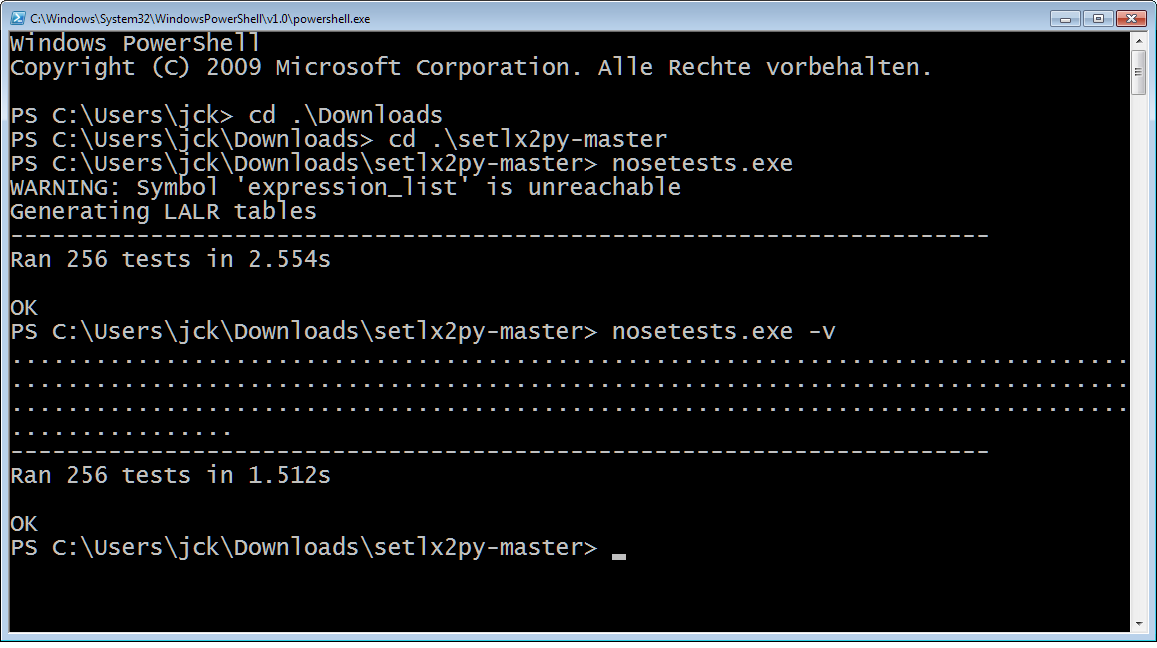
\includegraphics[width=0.8\textwidth]{img/run-nose.png}
	\caption{Output of nosetest: All tests passed}

\end{figure}
%!TEX root = ../main.tex

\section{AST}
\label{sec:ast}

The nodes for the \gls{ast} used  internally are generated from a config file to ease development. For the purpose of this project, the AST-generating part of another open-source compiler project\footnote{\url{https://github.com/eliben/pycparser}}  was forked into another project \footnote{\url{https://github.com/Rentier/ast-gen}} for that. New functionallity was added to ease testing them against expected trees.  Further more, their vizualization was improved.

The idea behind ast-gen is to describe the nodes, their attributes and children in a config file. From it, a Python file containing one class for every node is generated and then can be used without any dependency to the ast-gen project. Therefore, it is only needed in development.

\subsection{Configuration}

Each entry in the config file is a sub-class \texttt{<name>} of Node, listing its attributes and child nodes. Each line contains the name of the class, followed by it attributes:

\verb$<Name>: [list, of, attributes]$

The attributes can be of the following kind:

\begin{verbatim}
<name>*     - a child node
<name>**    - a sequence of child nodes
<name>      - an attribute.
\end{verbatim}

Example:

\begin{verbatim}
BinaryOp: [op, left*, right*]
Constant: [type, value]
ExprList: [exprs**]
\end{verbatim}

The file used in setlx2py can be found in \texttt{setlx2py/setlx_ast.cfg}.

\subsection{Generation}

After installing ast-gen, the Python file can be generated with the folling command in a Python shell:

\begin{lstlisting}{language=python}
from astgen.ast_gen import ASTCodeGenerator
gen = ASTCodeGenerator(**PATH_TO_CONFIG.cfg**)
with open(**PATH_TO_WHERE_TO_SAVE**, 'w') as f:
gen.generate(f)
\end{lstlisting}

Alternatively, the Makefile delivered with setlx2py offers a nice shortcut:

\verb$make ast$
%!TEX root = ../main.tex

\section{Code generation}

\label{sec:codegen}
%!TEX root = ../main.tex

\section{Transformation}

\label{sec:transformer}

In order to make code generation easier, the parser-generated AST is partially rewritten.  Mostly, that is done because some constructs in SetlX and Python differ quite largely. This maybe could also be done in the parser, but the main reason for a dedicated transformation step is to decouple the components. 

It was tried to avoid altering the parser in order to simplify code generation, as these components should be as simple an as´independent from each other as possible. 

The implementation is similar to the one of code generation: the AST is traversed depth-first, and one can specify actions for every AST node type. 

In this section, the two most interesting and complex cases are described.

%
\subsection{Procedure definitions}

In order to define a function in SetlX, one creates an anonymous function and binds it to a name via assignment.

\begin{lstlisting}[language=c]
signum := procedure(n) {
    if(n > 0) {
        return 1;
    } else if(n < 0) {
        return - 1;
    } else {
        return 0;
    }
};
\end{lstlisting}

In Python, when defining a function, it is automatically bound to that name in the current scope:

\begin{lstlisting}[language=python]
def signum(n):
    if n > 0:
        return 1
    elif n < 0:
        return - 1;
    else:
        return 0;
\end{lstlisting}

The AST for a procedure definition in setlx2py consists of the assignment node itself with name on the left- and the procedure on the right-hand side. As an example, the following procedure is discussed:

\begin{lstlisting}[language=c]
add := procedure(a,b) { return a + b; };
\end{lstlisting}

The corresponding AST is

\begin{lstlisting}[language=lisp]
('Assignment', ':=', 
  ('Identifier', 'add'), 
  ('Procedure', '', 'vanilla', 
    ('ParamList', ('Param', 'a'), ('Param', 'b')), 
    ('Block', 
      ('Return', 
        ('BinaryOp', '+', 
          ('Identifier', 'a'), 
          ('Identifier', 'b'))))))
\end{lstlisting}

One can see that the name of the procedure, (which Python needs for declaring it) is to be found in the assignment node. In the code generation step, only the current node and is children are visible to a callback. That means, the procedure node would have no access to the procedure name. The simple solution is to rewrite the AST for this construct. The rule for that is therefore that if there is an assignment statement where the right-hand side is a procedure, the name is assigned to the procedure node and the assignment node is replaced with its right-hand side:

\begin{lstlisting}[language=python]
def visit_Assignment(self, n, p):
    if isinstance(stmt, Assignment) and isinstance(stmt.right, Procedure):
        assignment = stmt
        procedure = assignment.right
        procedure.name = assignment.target.name
        n.stmts[i] = procedure
\end{lstlisting}

The result of transformation is

\begin{lstlisting}[language=lisp]
('Procedure', 'add', 'vanilla', 
  ('ParamList', ('Param', 'a'), ('Param', 'b')), 
  ('Block', 
    ('Return', 
      ('BinaryOp', '+',
        ('Identifier', 'a'), 
        ('Identifier', 'b')))))
\end{lstlisting}

\todo{Update to rewritten visit\_Assignment}

%
\subsection{Interpolation}

String interpolation in SetlX offers an easy way to inline expressions into strings. It is especially a nice syntax to create strings from data. 

\begin{lstlisting}
s := "signum($n$) is $signum(n)$.";
\end{lstlisting}

As a string is enriched with expressions, these have to be parsed aswell. Therefore, interpolation is only available at compile time. Parsing of the inlined expressions is done after the AST has been generated by the parser. To be more specific, it is done in the transformation phase. The high-level view is very simple:

\begin{lstlisting}[language=python]
def visit_Interpolation(self, n, p):
    self.fill_interpolation(n)
    self.generic_visit(n, p)
\end{lstlisting}

The \token{fill_interpolation} extracts the expressions in the given string, parses them, and creates the string format with the expressions as arguments. The AST after parsing is

\begin{lstlisting}[language=lisp]
('Assignment', ':=', 
  ('Identifier', 's'), 
    ('Interpolation', 
      ('Constant', 'literal', 'signum($n$) is $signum(n)$.'), 
      ('ExprList',)))
\end{lstlisting}

The result of transformation is

\begin{lstlisting}[language=lisp]
('Assignment', ':=', 
  ('Identifier', 's'), 
  ('Interpolation', 
    ('Constant', 'literal', 'signum({0}) is {1}.'), 
    ('ExprList', 
      ('Identifier', 'n'), 
      ('Call', 
        ('Identifier', 'signum'), 
        ('ArgumentList', 
          ('Identifier', 'n'))))))
\end{lstlisting}

Finally, the generated Python code is 

\begin{lstlisting}
s = "signum({0}) is {1}.".format(n, signum(n))
\end{lstlisting}


\section{Known issues}

There is still work to be done:

\subsection{Missing statements}

\begin{itemize}
  \item Scan
  \item Try/Catch
  \item Backtrack
\end{itemize}

\subsection{Missing features}

\begin{description}
  \item[Omega] Currently, the null literal \texttt{om} is not yet implemented. It should be easily matched by Pythons \texttt{None}, but there was no documentation about \texttt{om}.
  \item[Builtins] The most important and most frequently used library functions were implemented, but many are still missing.
\end{description}

\subsection{Defective features}

The datastructures have to be much more tested. Currently, all unit tests taken from the SetlX guide pass, but the set, especially as a relation and with builtin functions called on it appears buggy. One can see that when SetlX example code containing it, like the queens problem is compiled and run.

% ************************
% SETLX2PY bibliography 
% ************************

\clearpage
\nocite{*}

\printbibliography 


\end{document}